% Copyright 2004 by Till Tantau <tantau@users.sourceforge.net>.
%
% In principle, this file can be redistributed and/or modified under
% the terms of the GNU Public License, version 2.
%
% However, this file is supposed to be a template to be modified
% for your own needs. For this reason, if you use this file as a
% template and not specifically distribute it as part of a another
% package/program, I grant the extra permission to freely copy and
% modify this file as you see fit and even to delete this copyright
% notice. 

\documentclass{beamer}
% Replace the \documentclass declaration above
% with the following two lines to typeset your 
% lecture notes as a handout:
%\documentclass{article}
%\usepackage{beamerarticle}


% There are many different themes available for Beamer. A comprehensive
% list with examples is given here:
% http://deic.uab.es/~iblanes/beamer_gallery/index_by_theme.html
% You can uncomment the themes below if you would like to use a different
% one:
%\usetheme{AnnArbor}
%\usetheme{Antibes}
%\usetheme{Bergen}
%\usetheme{Berkeley}
%\usetheme{Berlin}
%\usetheme{Boadilla}
%\usetheme{boxes}
%\usetheme{CambridgeUS}
%%\usetheme{Copenhagen}
%\usetheme{Darmstadt}
%\usetheme{default}
%\usetheme{Frankfurt}
%\usetheme{Goettingen}
%\usetheme{Hannover}
%\usetheme{Ilmenau}
%\usetheme{JuanLesPins}
%\usetheme{Luebeck}
%\usetheme{Madrid}
%\usetheme{Malmoe}
\usetheme{Marburg}
%\usetheme{Montpellier}
%\usetheme{PaloAlto}
%\usetheme{Pittsburgh}
%\usetheme{Rochester}
%\usetheme{Singapore}
%\usetheme{Szeged}
%\usetheme{Warsaw}

%\usecolortheme{seahorse}
\setbeamertemplate{blocks}[rounded][shadow=true]
\setbeamertemplate{navigation symbols}{}

\setbeamercolor{section in sidebar}{fg=yellow}
\setbeamercolor{subsection in sidebar}{fg=yellow}
\setbeamercolor{author in sidebar}{fg=green}
\setbeamercolor{block body}{bg=normal text.bg!90!black}
\setbeamercolor{block title}{bg=blue,fg=white}
\setbeamercolor{block body example}{bg=normal text.bg!90!black}
\setbeamercolor{block title example}{bg=black,fg=white}
\setbeamercolor{block body alerted}{bg=normal text.bg!90!black}
\setbeamercolor{block title alerted}{bg=red,fg=white}

\title{Algorithmic Game Theory}

% A subtitle is optional and this may be deleted
\subtitle{Basic Solution Concepts and Computational Issues}

\author{Karel~Ha}
% - Give the names in the same order as the appear in the paper.
% - Use the \inst{?} command only if the authors have different
%   affiliation.

%\institute[Universities of Somewhere and Elsewhere] % (optional, but mostly needed)
%{
%  Department of Applied Mathematics\\
%  Charles University
%}
% - Use the \inst command only if there are several affiliations.
% - Keep it simple, no one is interested in your street address.

\date{Spring School of Combinatorics 2014}
% - Either use conference name or its abbreviation.
% - Not really informative to the audience, more for people (including
%   yourself) who are reading the slides online

\subject{Theoretical Computer Science}
% This is only inserted into the PDF information catalog. Can be left
% out. 

% If you have a file called "university-logo-filename.xxx", where xxx
% is a graphic format that can be processed by latex or pdflatex,
% resp., then you can add a logo as follows:

% \pgfdeclareimage[height=0.5cm]{university-logo}{university-logo-filename}
% \logo{\pgfuseimage{university-logo}}

% Delete this, if you do not want the table of contents to pop up at
% the beginning of each subsection:
%\AtBeginSubsection[]
%{
%  \begin{frame}<beamer>{Outline}
%    \tableofcontents[currentsection,currentsubsection]
%  \end{frame}
%}

\newcommand{\R}{\mathbb{R}}
\newtheorem{proposition}{Proposition}

% Let's get started
\begin{document}

\begin{frame}
  \titlepage
\end{frame}

\begin{frame}{Outline}
  \tableofcontents[pausesections]
  % You might wish to add the option [pausesections]
\end{frame}

% Section and subsections will appear in the presentation overview
% and table of contents.
\section{Motivational examples}

\subsection{The Prisoner's Dilemma}

%\begin{frame}{First Slide Title}{Optional Subtitle}
%  \begin{itemize}
%  \item {
%    My first point.
%  }
%  \item {
%    My second point.
%  }
%  \end{itemize}
%\end{frame}

\begin{frame}{The Prisoner's Dilemma}
  \begin{center}
    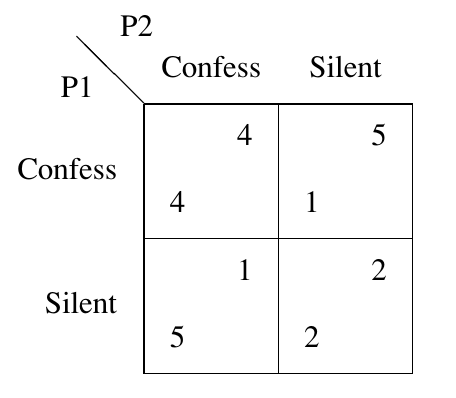
\includegraphics[width=\textwidth,height=0.8\textheight,keepaspectratio]{img/prisoner.png}
  \end{center}
\end{frame}

\begin{frame}{ISP routing game}
  \begin{center}
    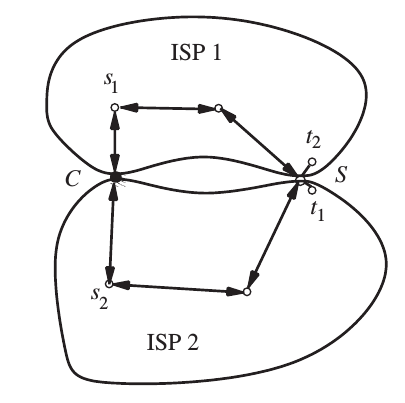
\includegraphics[width=\textwidth,height=0.8\textheight,keepaspectratio]{img/isp.png}
  \end{center}
\end{frame}

\subsection{Tragedy of the Commons}

\begin{frame}{Pollution game}{multiplayer version of Prisoner's dilemma}
  \pause
  \begin{itemize}
    \item $n$ countries
      \pause
    \item to \emph{control} pollution or \emph{not} to
      \pause
    \item to control $\mapsto$ cost of $3$ 
      \pause
    \item not to control $\mapsto$ adds $1$ to the cost of all countries
      \pause
  \end{itemize}
\end{frame}

% You can reveal the parts of a slide one at a time
% with the \pause command:
%\begin{frame}{Second Slide Title}
%  \begin{itemize}
%  \item {
%    First item.
%    \pause % The slide will pause after showing the first item
%  }
%  \item {   
%    Second item.
%  }
%  % You can also specify when the content should appear
%  % by using <n->:
%  \item<3-> {
%    Third item.
%  }
%  \item<4-> {
%    Fourth item.
%  }
%  % or you can use the \uncover command to reveal general
%  % content (not just \items):
%  \item<5-> {
%    Fifth item. \uncover<6->{Extra text in the fifth item.}
%  }
%  \end{itemize}
%\end{frame}

\subsection{Coordination games}

%\begin{frame}{Battle of the sexes}
%  \begin{center}
%    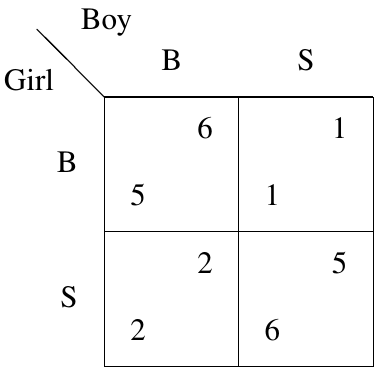
\includegraphics[width=\textwidth,height=0.8\textheight,keepaspectratio]{img/battle-of-sexes.png}
%  \end{center}
%\end{frame}

\begin{frame}{Routing congestion game}
  \begin{center}
    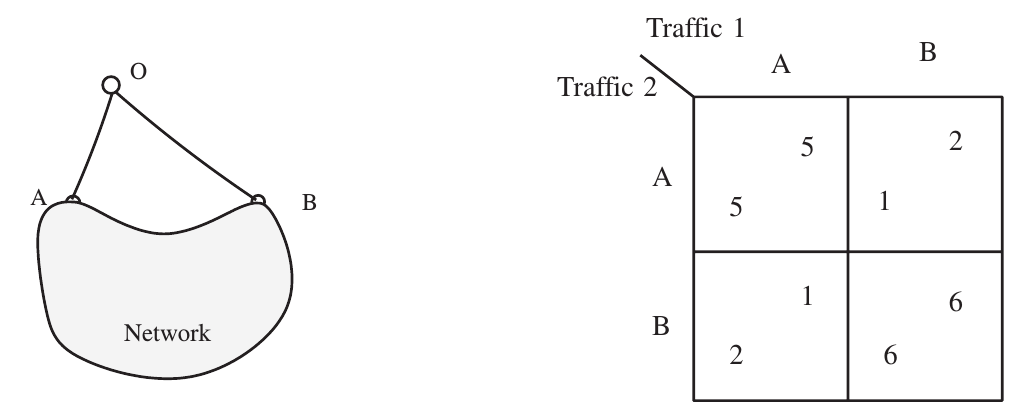
\includegraphics[width=\textwidth,height=0.8\textheight,keepaspectratio]{img/routing-congestion-game.png}
  \end{center}
\end{frame}

\section{Definitions}

\begin{frame}{Simultaneous move game}
  \begin{itemize}
      \pause
    \item set $N$ of players $\{1, 2, \dots, n\}$
      \pause
    \item each player $i$'s own set of possible {\bf pure} strategies $S_i$,
      from which a~strategy $s_i\in S_i$ is selected
      \pause
    \item the {\bf outcome} determined by the vector of selected strategies
      $s\in S_1\times\dots\times S_n =: S$
      \pause
      \begin{itemize}
        \item preference ordering on these outcomes: a complete, transitive,
          reflexive binary relation (on the set of all strategy vectors)
          \pause
        \item the {\bf payoff} (utility) $u_i:S\to \R$ to each player $i$, or
          {\bf cost} $c_i:S\to \R$ in other games
          \pause
      \end{itemize}
  \end{itemize}
\end{frame}

\begin{frame}{Representations of games}
  \pause

  {\bf Standard (matrix) form}
  \begin{itemize}
    \item given by the list of all possible strategy combinations together with
      respective payoffs
  \end{itemize}

  \pause
  {\bf Compactly represented game}
  \begin{itemize}
    \item a~succinct formulation rather than the explicit one
      \pause
    \item for example, the formula in the Pollution game
  \end{itemize}

\end{frame}

\section{Solution concepts}

\subsection{Dominant strategy}

\begin{frame}{Dominant strategy}
  It is the strategy vector $s\in S$ such that for each player $i$ and each
  alternate strategy vector $s'\in  S$, we have that
  \[u_i(s_i, s'_{-i})\ge  u_i(s'_i, s'_{-i}),\]
  where $s_{-i}$ denotes the strategy vector $s$ without the $i$-th stra\-te\-gy
  $s_i$.

  \begin{center}
    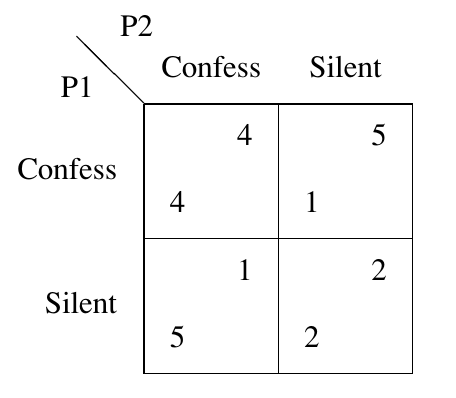
\includegraphics[width=\textwidth,height=0.5\textheight,keepaspectratio]{img/prisoner.png}
  \end{center}
\end{frame}

\subsection{Nash equilibria}

\begin{frame}{Pure Nash equilibrium}
  It is the strategy vector $s\in S$ such that for each player $i$ and each
  alternate strategy $s'_i\in  S_i$ we have that
  \[u_i(s_i, s_{-i})\ge  u_i(s'_i, s_{-i}).\]

  \begin{center}
    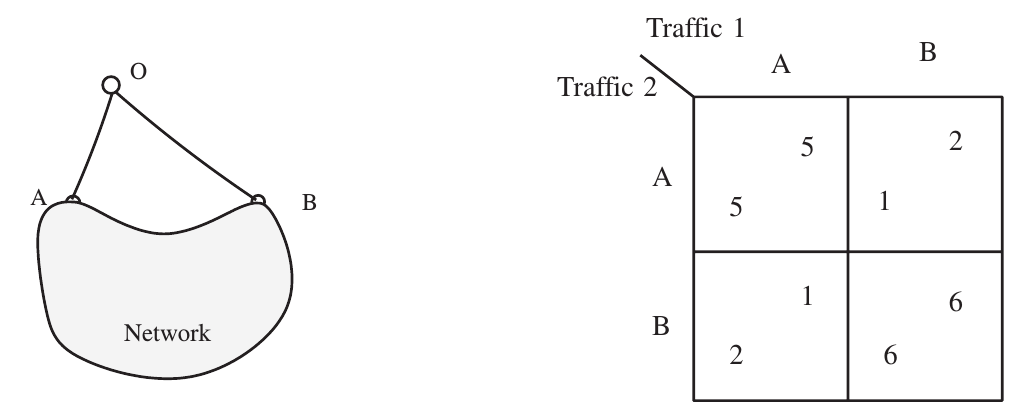
\includegraphics[width=\textwidth,height=0.8\textheight,keepaspectratio]{img/routing-congestion-game.png}
  \end{center}

  \pause
  Clearly, every dominant strategy is a~pure Nash equilibrium.

\end{frame}

\begin{frame}{Matching pennies}
  \begin{center}
    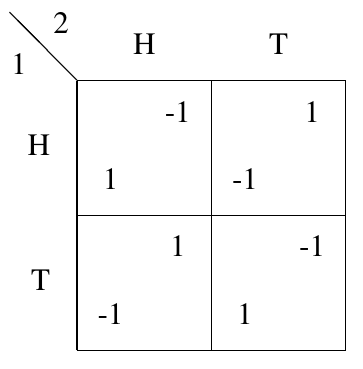
\includegraphics[width=\textwidth,height=0.8\textheight,keepaspectratio]{img/matching-pennies.png}
  \end{center}
\end{frame}

\begin{frame}{Mixed strategy}
  A {\bf mixed strategy $m_i:S_i\to[0,1]$} of player $i$ is a probabilistic
  distribution over the set $S_i$.
  \pause

  Each player $i$ thus aims to maximize the expected payoff $\bar u_i(m_i, m_{-i})$
  under this distribution.

  \pause
  \begin{center}
    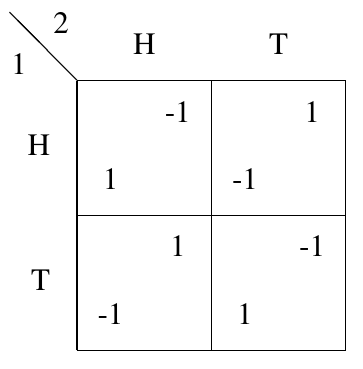
\includegraphics[width=\textwidth,height=0.6\textheight,keepaspectratio]{img/matching-pennies.png}
  \end{center}
\end{frame}

\begin{frame}{Mixed Nash equilibrium}
  A vector $m=(m_1,\dots,m_n)$ of mixed strategies of all players is called
  {\bf mixed Nash equilibrium} if for each player $i$ and each alternate mixed
  strategy $m'_i$ we have that 
  \[\bar u_i(m_i,m_{-i})\ge \bar u_i(m'_i,m_{-i}).\]
  \pause

  \begin{theorem}[Nash, 1951]
    Any game with a finite set of players and finite set of strategies has a
    mixed Nash equilibrium.
  \end{theorem}

  %\pause
  %Are the conditions of finiteness necessary?
  %\pause
  %- Yes!!
\end{frame}

%\begin{frame}{Pricing game}
%  \begin{center}
%    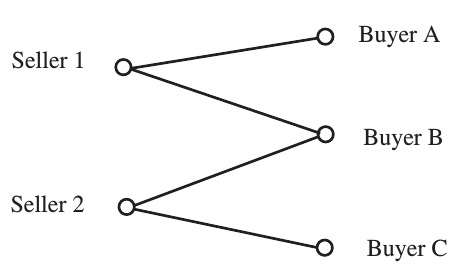
\includegraphics[width=\textwidth,height=0.8\textheight,keepaspectratio]{img/pricing-game.png}
%  \end{center}
%\end{frame}

\subsection{Correlated equilibrium}

\begin{frame}{Traffic light}
  \begin{center}
    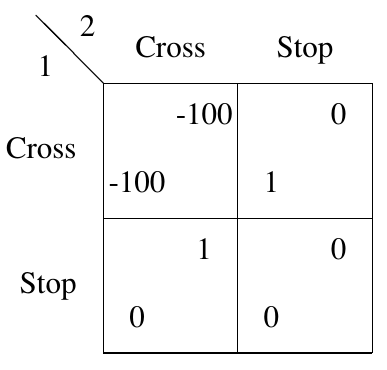
\includegraphics[width=\textwidth,height=0.8\textheight,keepaspectratio]{img/traffic-light.png}
  \end{center}
\end{frame}

\begin{frame}{Correlated equilibrium}
  An external correlation device suggests a~strategy vector $s$ with the
  probability $p(s) = p(s_i, s_{-i})$.
  \pause

  A {\bf correlated equilibrium} is a probability distribution $s$ over
  strategy vectors such that for each player $i$ and each alternate strategy
  $s'_i$ we have that
  \[\sum_{s_{-i}} p(s_i , s_{-i}) u_i(s_i , s_{-i}) \ge \sum_{s_{-i}} p(s'_i ,
    s_{-i}) u_i(s'_i , s_{-i}).\]
\end{frame}

\section{Finding Equilibria}

\begin{frame}{PPAD complexity class}{Polynomial Parity Argument (Directed case)}
  Examples of problems
  \pause
  \begin{itemize}

    \item cutting Ham Sandwiches
      \begin{itemize}
        \item Given $n$ sets of $2n$ points each in $n$ dimensions, find a
          hyperplane which, for each of the $n$ sets, leaves $n$ points on each
          side.
      \end{itemize}
  \pause

    \item finding Brouwer and Borsuk-Ulam fixpoints
  \pause

    \item finding Arrow-Debreu equilibria in markets
  \pause
  \end{itemize}
  See Papadimitriou (1994) for details.
\end{frame}

\begin{frame}{Complexity of finding Nash equilibrium}
  \pause
  \begin{theorem}
    Finding Nash equilibrium is PPAD-complete.
  \end{theorem}

  \pause
  \structure{Proof.} \\
    Chapter 2 of Nisan, Roughgarden, Tardos, Vazirani: \emph{Algorithmic Game
      Theory}.
    \qed
\end{frame}

\begin{frame}{Two-Person Zero-Sum Games}{The sum of the payoffs of the two
    players is zero for any choice of strategies.}
  \pause
  \begin{itemize}
    \item payoff matrix $A$ (for the row player)
  \pause
    \item Nash equilibrium: row vector $p^*$, column vector $q^*$ 
  \pause
    \item expected payoff equals $v^* = p^*Aq^*$
  \pause
  \end{itemize}

  \begin{proposition}
    Two-Person Zero-Sum Games can be solved via the linear programming.
  \end{proposition}
\end{frame}

\begin{frame}{The proof}{Episode I}
  \begin{itemize}
    \item In a Nash equilibrium, even if a player knows the strategies of
      others, he cannot be better off by deviating.
      \pause
    \item If the row player's strategy $p$ was publicly known, the column
      player would want to minimize his loss.
      \pause
    \item Hence, he would choose the minimum entries in $pA$.
      \pause
    \item So the best publicly announced strategy (for the row player) is to
      maximize this minimum value.
      \pause
  \end{itemize}
\end{frame}

\begin{frame}{The proof}{Episode II}
  \begin{align*}
    v_r :&= \textrm{max} \; v \\
    \sum_{i} p_i &= 1 \\
    p &\geq 0 \\
    (pA)_j &\geq v \; \textrm{for all} \; j\\
  \end{align*}
    \pause
  \begin{itemize}
    \item The row player can guarantee to win at least $v_r$ in any
      equilibrium, therefore $v_r \leq v^*$.
    \pause
    \item An equilibrium is stable even if known to the opponent, therefore
      $v^* \leq v_r$.
    \pause
    \item Thus $v^* = v_r$.
  \end{itemize}
\end{frame}

\begin{frame}{The proof}{Episode III}
  Similarly, for the linear program (of the column player)
  \begin{align*}
    v_c :&= \textrm{min} \; v \\
    \sum_{j} q_j &= 1 \\
    q &\geq 0 \\
    (Aq)_i &\leq v \; \textrm{for all} \; i\\
  \end{align*}
  we have that $v^* = v_c$, and therefore, $v_r = v_c$.
  \pause

  Optimal solutions $p_r$ and $q_c$ to the two linear programs form a Nash
  equilibrium.
  \qed

  \pause
  \vskip .25cm
  Note that the programs are duals of each other.
\end{frame}

\begin{frame}
  \begin{center}
    Thank you!
  \end{center}
\end{frame}

\appendix
\section*{Games with turns}

\begin{frame}{Ultimatum game}
  \pause
  \begin{itemize}
    \item seller $S$, buyer $B$
      \pause
    \item 2 steps:
      \begin{itemize}
        \item $S$ offers price $p$
        \item $B$ reacts
      \end{itemize}
      \pause
    \item $S$ has payoff $p$ if the sale occurs, and $0$ otherwise.
      \pause
    \item $B$ has a value $v$ for the good and he has payoff $v-p$ if he buys,
      and $0$ otherwise.
      \pause
    \item $S$ is aware of $B$'s value $v$ (full information game).
  \end{itemize}
\end{frame}
%
%\begin{frame}{Subgame Perfect Equilibrium}
%  In the Ultimatum game the notion of Nash equilibrium seems weak.
%\end{frame}
%
%%\section*{The End}
%%\begin{frame}
%%  \begin{center}
%%    Thank you!
%%  \end{center}
%%\end{frame}
%
%%\subsection{Another Subsection}
%%
%%\begin{frame}{Blocks}
%%\begin{block}{Block Title}
%%You can also highlight sections of your presentation in a block, with it's own title
%%\end{block}
%%\begin{theorem}
%%There are separate environments for theorems, examples, definitions and proofs.
%%\end{theorem}
%%\begin{example}
%%Here is an example of an example block.
%%\end{example}
%%\end{frame}
%
%% Placing a * after \section means it will not show in the
%% outline or table of contents.
%%\section*{Summary}
%%
%%\begin{frame}{Summary}
%%  \begin{itemize}
%%  \item
%%    The \alert{first main message} of your talk in one or two lines.
%%  \item
%%    The \alert{second main message} of your talk in one or two lines.
%%  \item
%%    Perhaps a \alert{third message}, but not more than that.
%%  \end{itemize}
%%  
%%  \begin{itemize}
%%  \item
%%    Outlook
%%    \begin{itemize}
%%    \item
%%      Something you haven't solved.
%%    \item
%%      Something else you haven't solved.
%%    \end{itemize}
%%  \end{itemize}
%%\end{frame}
%
%
%
%% All of the following is optional and typically not needed. 
%\appendix
%\section{Optional \appendixname}
%\subsection{Markets and Their Algorithmic Issues}
%
%\begin{frame}{An Algorithm for a Simple Market}
%\end{frame}
%
%\subsection<presentation>*{For Further Reading}
%
%\begin{frame}[allowframebreaks]
%  \frametitle<presentation>{For Further Reading}
%    
%  \begin{thebibliography}{10}
%    
%  \beamertemplatebookbibitems
%  % Start with overview books.
%
%  \bibitem{Author1990}
%    A.~Author.
%    \newblock {\em Handbook of Everything}.
%    \newblock Some Press, 1990.
% 
%    
%  \beamertemplatearticlebibitems
%  % Followed by interesting articles. Keep the list short. 
%
%  \bibitem{Someone2000}
%    S.~Someone.
%    \newblock On this and that.
%    \newblock {\em Journal of This and That}, 2(1):50--100,
%    2000.
%  \end{thebibliography}
%\end{frame}

\end{document}


